\documentclass[10pt,xetex]{beamer} %[compress, blue]
\mode<presentation>


\date{\today}
\title{Lexicography and morphology
    \scriptsize{ESU-DH in Leipzig 2018-07}}

\begin{document}

\section{Introduction}

\begin{frame} %% framesection
 \begin{center}
 {\Large {\bf Introduction}}  % Introduction
 \end{center}
\end{frame}

\begin{frame}
  \frametitle{Introduction}

In this talk I am doing to talk about:

\begin{itemize}
  \item What we mean by {\em morphology}
  \item Which parts of morphology we are interested in
  \item How morphology is represented with {\em computers}
  \item Examples of phenomena in different language and how we can treat them
\end{itemize}

At the end of this talk you should have an idea of:

\begin{itemize}
  \item How morphology is represented in HFST and lttoolbox
  \item How to treat different morphological phenomena in these formalisms
\end{itemize}

\end{frame}

\begin{frame}
  \frametitle{What is morphology?}

Morphology is: ~\\
~\\

 « the branch of linguistics that studies patterns of word formation within and
 across languages, and attempts to formulate rules that model the knowledge
 of the speakers of those languages. »\\
~\\

This is a big field, in MT we are only interested in a part of it.

\end{frame}

\begin{frame}
  \frametitle{Why ?}

So why do we want to do morphology ?  \\
\begin{itemize}
    \item Sometimes it's just easier to deal with rules than listing everything:
    \item<2> Sometimes it's actually kind of sort of necessity to be able to
        generate all forms with rules and not list everything...:
\end{itemize}
\only<1>{
    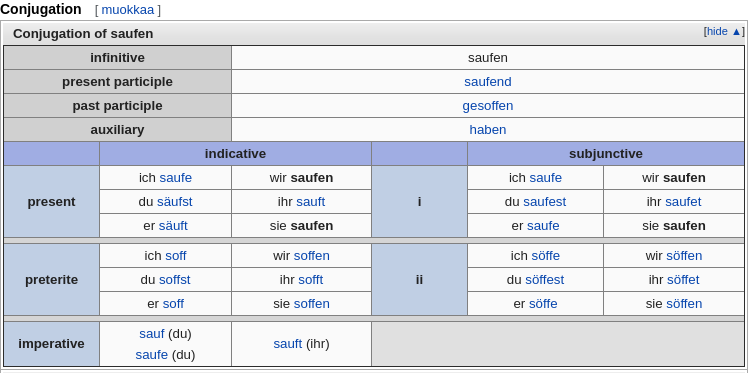
\includegraphics[width=.8\textwidth]{wiktionary-morphs}
}\only<2>{
    
\includegraphics[width=.8\textwidth]{omorfi-forms}
}
\end{frame}

\begin{frame}
  \frametitle{Morphology in machine translation}

In machine translation we are interested in building and using computational
models of morphology for {\em translation}.

We are interested in being able to do the following things:

\begin{itemize}
 \item {\bf Tokenisation}: Split text into units consisting of words
 \begin{itemize}
     \item pitää tietää, mitä käännetään. $\rightarrow$ $[$pitää$]$ $[$tietää$]$
         $[$,$]$ $[$mitä$]$ $[$käännetään$]$ $[$.$]$
 \end{itemize}
\item {\bf Analysis}: Analysing these words, giving for each one a list of
    possible interpretations / morphological descriptions
  \begin{itemize}
    \item runs $\rightarrow$ {\tt run+verb.p3.sg}, {\tt run+noun.pl},
  \end{itemize}
\item {\bf Generation}: Given a morphological description of a word generate the
    corresponding surface form.
  \begin{itemize}
    \item {\tt dürfen+verb.pres.p3.sg} $\rightarrow$ darg
  \end{itemize}
\end{itemize}

\end{frame}

\begin{frame}
  \frametitle{Morphotactics and morphophonology}

\begin{itemize}
  \item {\bf Morphotactics}:
  \begin{itemize}
    \item How morphemes (units of meaning) are arranged to form words
      \begin{itemize}
        \item Example: {\tt роза<n><pl><gen>} $\rightarrow$ роз(а) + Ø
       \item Example: {\tt розетка<n><pl><gen>} $\rightarrow$ розетк(а) + Ø
      \end{itemize}
  \end{itemize}
  ~\\
  \item {\bf Morphophonology}:
  \begin{itemize}
    \item Phonological changes that happen when morphemes are joined together
    \begin{itemize}
      \item Example: роз(а) + Ø $\rightarrow$ роз
      \item Example: розетк(а) + Ø $\rightarrow$ розеток
      \item ~~~~(а) $\rightarrow$ о: between final тк, add; otherwise, don't
    \end{itemize}
  \end{itemize}
\end{itemize}

This session focusses on morphotactics

\end{frame}

%%%%%%%%%%%%%%%%%%%%%%%%%%%%%%%%%%%%%%%%%%%%%%%%%%%%%%%%%%%%%%%%%%%%%%%%%%%%%%%
%%
%%%%%%%%%%%%%%%%%%%%%%%%%%%%%%%%%%%%%%%%%%%%%%%%%%%%%%%%%%%%%%%%%%%%%%%%%%%%%%%

\begin{frame} %% framesection
 \begin{center}
 {\Large {\bf Morphotactics}}
 \end{center}
\end{frame}

\begin{frame}
  \frametitle{Morphotactics}

So, as mentioned previously, morphotactics is how we describe how morphemes
are put together to form words. This can be further divided into several
subprocesses:

\begin{itemize}
  \item {\bf Inflection}: Inflectional morphemes carry grammatical information, such as number, case, tense, etc., but do not change the word category
  \item {\bf Derivation}: Derivational morphemes change the basic semantic meaning of a word, and can also change word category.
  \item {\bf Compounding}: Compounding is a process where two or more words are joined together to form one.
  \item {\bf Clitics}: A clitic is a syntactically independent word that functions phonologically as an affix of another word.
\end{itemize}

There is another relevant process for machine translation which is related,

\begin{itemize}
  \item {\bf Multiword units}: A multiword unit is a set of words which should be treated for the purposes of a given natural language processing task as a single word.
\end{itemize}

\end{frame}

\begin{frame}
  \frametitle{Inflection}

Here are some examples of inflection:

\begin{itemize}
  \item {\bf Case suffixes}: работ·а, работ·ы, работ·е; ӗҫ·ӗн, ӗҫ·е, ӗҫ·ре
  \item {\bf Plural suffixes}: ӗҫ·сем
  \item {\bf Possessive suffixes}: ӗҫ·ӗм, ӗҫ·ӳ, ӗҫ·ӗ
  \item {\bf Tense, aspect and mood suffixes}: работ·аю, работ·аешь; ӗҫ·л·ет·ӗп, ӗҫ·л·ет·ӗн, ӗҫ·ле·м··ӗп, ӗҫ·ле·м··ӗн
  \item {\bf Comparison suffixes}: бел·ее, боль·ш·е; шур·рах, пысăк·рах, ĕç·чен·рех
\end{itemize}

\end{frame}

\begin{frame}
  \frametitle{Derivation}

% !!warning!!
% anti-dis-establish-ment-ari-an-ism
% `the ideology of the opposition to the separation of church and state'
% we're interested in what we cantranslate!!

Here are some examples of derivation:

\begin{itemize}
  \item {\bf Actor suffixes}: работ·ник, специал·ист; ĕç·чен, ĕç·ле·кен % Actor suffixes
  \item {\bf State suffixes}: бед·н·ость, свеж·есть, велич·ина % State suffixes
  \item {\bf Causative suffixes}: ĕç·ле·ттер % Causative suffixes
\end{itemize}

Derivation is interesting to model from a morphology/grammar point of view,
but care should be taken when trying to model it in translation

\end{frame}

\begin{frame}
  \frametitle{Warning: Derivation}

There are some things to take into account when dealing with derivation from
a machine translation perspective. The most important is:

\begin{center}
   {\bf Can you translate it predictably?}
\end{center}

If the answer to this question is no, then it might be better to {\em lexicalise}
the stem + derivation as a separate stem. An examples might be:

\begin{itemize}
  \item Actor suffix {\em -er} in English: Often ambiguous between person and machine:
  \begin{itemize}
     \item cook + er = machine that cooks
     \item clean + er = person who cleans
     \item look + er = person that looks (is seen to look) {\em good}
  \end{itemize}
\end{itemize}

Some derivations may be possible with some words, but not others, and may be ambiguous with other, non-derived, forms:

\begin{itemize}
  \item driver + er = driver, walk + er = walker, vote + er = voter
  \item wash + er = *washer (but potwasher), plough + er = *plougher
\end{itemize}

\end{frame}

\begin{frame}
  \frametitle{Compounding}

Compounding is fairly straightforward, morphologically/syntactically independent words are placed together to form new words.

\begin{itemize}
  \item This may be indicated in the writing system or not.
  \begin{itemize}
    \item infrastruktuurontwikkelingsplan, or
    \item infrastructure development plan
  \end{itemize}
  \item Both are noun-noun-noun compounds, but they are treated differently by the respective writing systems
\end{itemize}

If the writing system of your language writes compounds together, then they probably need to be treated in your morphological analyser.

However, a given compound word may be split different ways, or a given word may appear as a compound, but not be one:

\begin{itemize}
  \item Freitag = Friday (not ``Frei'' + ``tag'' = free day)
  \item kulturforskeren = the ethnographer, а not
  \begin{itemize}

  \item kultur+forskeren = ``culture researcher''
  \item kultur+forske+ren = ``culture research clean''
  \end{itemize}
\end{itemize}

\end{frame}
%
%\begin{frame}
%  \frametitle{Multiwords}
%
%We'll talk about multiwords in Session 2
%
%
%\end{frame}

%%%%%%%%%%%%%%%%%%%%%%%%%%%%%%%%%%%%%%%%%%%%%%%%%%%%%%%%%%%%%%%%%%%%%%%%%%%%%%%
%%
%%%%%%%%%%%%%%%%%%%%%%%%%%%%%%%%%%%%%%%%%%%%%%%%%%%%%%%%%%%%%%%%%%%%%%%%%%%%%%%

\begin{frame} %% framesection
 \begin{center}
 {\Large {\bf Computational morphology}}
 \end{center}
\end{frame}

\begin{frame}
  \frametitle{Computational morphology}

Now we've looked at various issues relating to morphology, we're going
to look at how to deal with them using computers. This section will look
at:

\begin{itemize}

  \item Finite-state transducers

  \item Lexicon formalisms ({\tt lttoolbox} and {\tt lexc})

  \item Tags

  \item Continuation lexica / paradigm

%  \item Flag diacritics

\end{itemize}

\end{frame}

\begin{frame}
  \frametitle{Finite-state transducers}

\begin{onlyenv}<1>
One way of modelling morphology is with a finite-state transducer,


\begin{itemize}
  \item A bit like a flowchart
  \item Has a set of states (questions) and transitions (decisions)
  \item Depending on the input, you make different decisions
\end{itemize}

This is much easier with an example:
\end{onlyenv}

\begin{onlyenv}<2>

\includegraphics[width=1.0\textwidth]{Bashkir-mektep.png}

\end{onlyenv}

\begin{onlyenv}<3>

So what are the benefits of using finite-state transducers, over for example
stemming or other rule-based, or database-based options?

\begin{itemize}
  \item The same code, and the same morphological description can be used for both analysis and generation
  \item The lookup time is linear (meaning they are {\em very} fast)
  \item Does not require programming knowledge
\end{itemize}

\end{onlyenv}

% what is a finite-state transducer

% benefits of finite-state transducers for modelling morphology
%  - two way -- the same code can be used for both analysis and generation
%  - linear lookup time

% drawbacks:
%  - complex morph. makes transducers get pretty big without special tricks

\end{frame}

\begin{frame}
  \frametitle{Lexicon formalisms}

In Apertium we have a couple of options when we want to make a new morphological description

\begin{itemize}
  \item {\bf lttoolbox}:
  \begin{itemize}
    \item The original lexicon format
    \item Based on XML
    \item One-level, morphotactics and morphophonology done in the same file
    \item More restrictive, but more userfriendly, e.g. comes with validation
    \item Useful features for MT built in (direction restrictions)
  \end{itemize}
  \item {\bf HFST lexc}:
  \begin{itemize}
    \item Very powerful, but no validation
    \item Can be one-level or two-level
    \item Text format
    \item Transducers can be cyclic
    %\item
  \end{itemize}
\end{itemize}

% lttoolbox
%  - for isolating and fusional languages
% HFST lexc
%  - for agglutinative and polysynthetic languages

\end{frame}
%
%\begin{frame}
%  \frametitle{Strengths and weaknesses}
%
%\begin{table}
%\begin{tabular}{l|l|l}
%                & Strengths  & Weaknesses \\
%\hline
%{\tt lttoolbox} &            & - \\
%\hline
%{\tt lexc}      &            & - \\
%\hline
%\end{tabular}
%\end{table}
%
%%           | strengths    | weaknesses
%% lttoolbox |              |
%% -----------------------------
%% lexc      |              |
%
%\end{frame}
%
\begin{frame}
  \frametitle{We recommend...}

\begin{itemize}
  \item {\bf lttoolbox} if you're working with isolating or fusional languages, e.g.
    \begin{itemize}
      \item Germanic languages
      \item Slavic languages
      \item Indo-Iranian languages
    \end{itemize}
  \item {\bf lexc} if you're working with agglutinative or polysynthetic languages, e.g.
    \begin{itemize}
      \item Turkic languages
      \item Uralic languages
      \item Caucasian languages
    \end{itemize}
\end{itemize}

But if you're going to use lexc, we have some coding practices that will make your life easier!

\end{frame}

\begin{frame}[fragile]
  \frametitle{General structure}

\begin{onlyenv}<1>
The general structure of both lttoolbox and lexc files is as follows:

\begin{itemize}

  \item First you define your tags

  \item Then you define your inflectional classes

  \item Then you define your lexicon

\end{itemize}
\end{onlyenv}

\begin{onlyenv}<2>
    \begin{verbatim}
<dictionary>
  <sdefs>
    <sdef n="n"   c="Noun"/>
    <sdef n="pl"  c="Plural"/>
    <sdef n="sg"  c="Singular"/>
  </sdefs>
  <pardefs>
    <pardef n="ninfl">
      <e><p><l/><r><s n="n"/><s n="sg"/></r></p></e>
      <e><p><l>\textbf{s}</l><r><s n="n"/><s n="pl"/></r></p></e>
    </pardef>
  </pardefs>
  <section id="Root" type="standard">
    <e lm="cat"><i>\textbf{cat}</i><par n="ninfl"/></e> <!-- A noun -->
  </section>
</dictionary>
    \end{verbatim}
\end{onlyenv}


\begin{onlyenv}<3>
\begin{verbatim}
Multichar_Symbols

%<n%>   ! Noun
%<pl%>  ! Plural
%<sg%>  ! Singular

LEXICON Root

NounRoot ;

LEXICON ninfl

%<n%>%<sg%>:   # ;
%<n%>%<pl%>:s   # ;

LEXICON NounRoot

cat ninfl ; ! A noun


\end{verbatim}

\end{onlyenv}
\end{frame}

\begin{frame}
  \frametitle{Tags} % Tags

{\bf tags} are special symbols, which denote grammatical features, a given analysis
from a morphological analyser will give a lemma (the dictionary form of the word),
and a sequence of tags, for example

\begin{itemize}
  \item Number: $<$sg$>$ = singular, $<$du$>$ = dual, $<$pl$>$ = plural \ldots
  \item Case: $<$nom$>$ = nominative, $<$abl$>$ = ablative, $<$ill$>$ = illative \ldots
  \item Tense: $<$pres$>$ = present, $<$past$>$ = past, $<$fut$>$ = future \ldots
\end{itemize}

In Apertium, tags are denoted by the less than $<$ and greater than $>$ characters

As we will see later, it is desirable that tags be as consistent as possible

\end{frame}

\begin{frame}
  \frametitle{Archiphonemes}

  {\bf archiphonemes} are special symbols which stand in place of a letter, they
    are handled by phonological rules, for example:

\begin{itemize}
  \item $\{$A$\}$ may be `a' or `ә' depending on the frontness/backness of the stem
  \item $\{$s$\}$ may be `с' or nothing depending on if the phoneme is preceeded by a vowel or a consonant
  \item $\{$k$\}$ may be `k' or `ğ' depending on if it is between vowels or not
\end{itemize}

In Apertium we write archiphonemes with \{ and \}\\
~\\

~~~~ More on this in Session 2!

\end{frame}


\begin{frame}[fragile]
  \frametitle{Continuation lexica / paradigms}

\begin{onlyenv}<1>
 A {\bf continuation lexicon} or {\bf paradigm} is a set of input/output pairs which defines an inflection class of a word

\begin{itemize}
  \item In an agglutinative language you may have a separate continuation lexica for each of a different set of suffixes, e.g. case, number, possession
  \item In a fusional language, typically a continuation lexicon will define the inflection pattern for a given word
\end{itemize}
\end{onlyenv}

\begin{onlyenv}<2>
%\begin{changemargin}{-1cm}{-1cm}
    \begin{verbatim}
{\smallermono
<pardef n="nan\_{}\_{}n\_{}ma">
<e><p><l></l><r><s n="n"/><s n="ma"/><s n="sg"/><s n="nom"/></r></p></e>
<e><p><l>\textbf{a}</l><r><s n="n"/><s n="ma"/><s n="sg"/><s n="gen"/></r></p></e>
<e><p><l>\textbf{ej}</l><r><s n="n"/><s n="ma"/><s n="sg"/><s n="dat"/></r></p></e>
<e><p><l>\textbf{a}</l><r><s n="n"/><s n="ma"/><s n="sg"/><s n="acc"/></r></p></e>
<e><p><l>\textbf{om}</l><r><s n="n"/><s n="ma"/><s n="sg"/><s n="ins"/></r></p></e>
<e><p><l>\textbf{je}</l><r><s n="n"/><s n="ma"/><s n="sg"/><s n="loc"/></r></p></e>
<e><p><l>\textbf{o}</l><r><s n="n"/><s n="ma"/><s n="sg"/><s n="voc"/></r></p></e>
 ...
</pardef>
}
\end{verbatim}
%\end{changemargin}
\end{onlyenv}

\begin{onlyenv}<3>
\vspace{-5pt}
\begin{verbatim}
LEXICON CLIT

%+мы%<qst%>:%>м%{I%} # ;
# ;

LEXICON CASE

%<nom%>: CLIT ;
%<dat%>:%>%{G%}%{A%} CLIT ;
%<acc%>:%>н%{I%} CLIT ;
...

LEXICON NUM

%<sg%>: CASE ;
%<pl%>:%>%{L%}%{A%}р CASE ;

LEXICON NLEX

%<n%>: NUM ;

\end{verbatim}
\end{onlyenv}


\end{frame}
%
%\begin{frame}
%  \frametitle{Flag diacritics}
%
%Sometimes it can be necessary to implement long distance dependencies in your analyser, for example
%
%\begin{itemize}
%  \item To model prefix or circumflex inflection
%  \item To disallow combinations of non-adjacent morphemes
%  \item ...
%\end{itemize}
%
%In {\bf lexc}, flag diacritics can be used for these purposes (more on that shortly)
%
%\end{frame}

\begin{frame}[fragile]
  \frametitle{Variants}

\begin{onlyenv}<1>
Another thing you might want to do when writing a morphological analyser is allow
for variants in the analysis, but only generate one form... for example,

\begin{itemize}
  \item Different standards: Analyse both ``analyse'' and ``analyze'', but only generate ``analyse''
  \item Irregular forms: Analyse both ``cherubim'' and ``cherubs'' but only generate ``cherubim''
\end{itemize}

\end{onlyenv}


\begin{onlyenv}<2>
\begin{verbatim}

<pardef n="anal/yse__vblex">
  <e><p><l>yse</l><r>yse<s n="vblex"/> ...
  <e r="LR"><p><l>yze</l><r>yse<s n="vblex"/> ...
</pardef>

...

<section id="main" type="standard">
  <e lm="analyse"><i>anal</i><par n="anal/yse__vblex"/></e>
</section>

\end{verbatim}
\end{onlyenv}

\begin{onlyenv}<3>
\begin{verbatim}

LEXICON VERB-YSE

%<vblex%>:yse # ;
%<vblex%>:yze # ; !Dir/LR

LEXICON Verbs

analyse:anal VERB-YSE ;

\end{verbatim}
\end{onlyenv}


\end{frame}



%%%%%%%%%%%%%%%%%%%%%%%%%%%%%%%%%%%%%%%%%%%%%%%%%%%%%%%%%%%%%%%%%%%%%%%%%%%%%%%
%%
%%%%%%%%%%%%%%%%%%%%%%%%%%%%%%%%%%%%%%%%%%%%%%%%%%%%%%%%%%%%%%%%%%%%%%%%%%%%%%%
%
%\begin{frame} %% framesection
% \begin{center}
% {\Large {\bf \cyrtext{Examples}}}
% \end{center}
%\end{frame}
%
%\begin{frame}
%  \frametitle{Examples}
%
%% i'd like to give some real life examples of how to deal with certain morphological
%%%  phenomena in lexc and lttoolbox
%
%% inflection - a typical way of creating noun inflection paradigms in fusional and
%%% agglutinative languages
%
%% derivation - how to do verb derivation in a turkic language
%
%% compounding - how to deal with compounding in fusional and agglutinative languages
%
%% clitics -  how to deal with clitics which are invariable, and those which change
%
%\end{frame}
%
%
%\begin{frame}
%  \frametitle{Example: Inflection}
%
%
%
%\end{frame}
%
%
%\begin{frame}
%  \frametitle{Example: Derivation}
%
%\end{frame}
%
%\begin{frame}
%  \frametitle{Example: Compounding}
%
%\end{frame}
%
%\begin{frame}
%  \frametitle{Example: Clitics}
%
%\end{frame}
%
%\begin{frame}
%  \frametitle{Example: Optional forms}
%\end{frame}
%
%%%%%%%%%%%%%%%%%%%%%%%%%%%%%%%%%%%%%%%%%%%%%%%%%%%%%%%%%%%%%%%%%%%%%%%%%%%%%%%
%%
%%%%%%%%%%%%%%%%%%%%%%%%%%%%%%%%%%%%%%%%%%%%%%%%%%%%%%%%%%%%%%%%%%%%%%%%%%%%%%%

\begin{frame} %% framesection
 \begin{center}
 {\Large {\bf Debugging and design}}
 \end{center}
\end{frame}

\begin{frame}[fragile]
  \frametitle{Debugging}

\begin{onlyenv}<1>

An important thing to be able to do when building a morphological description
is debugging, one of the most useful tools in both {\bf lttoolbox} and {\bf HFST}
is the ability to be able to print out all forms recognised by your description:

\end{onlyenv}

\begin{onlyenv}<2>
\begin{center}
{\bf lt-expand}
\end{center}
 \begin{verbatim}

$ lt-expand hsb.dix
nan:nan<n><ma><sg><nom>
nana:nan<n><ma><sg><gen>
nanej:nan<n><ma><sg><dat>
nana:nan<n><ma><sg><acc>
nanom:nan<n><ma><sg><ins>
nanje:nan<n><ma><sg><loc>
nano:nan<n><ma><sg><voc>
nanaj:nan<n><ma><du><nom>
nanow:nan<n><ma><du><gen>
\end{verbatim}

\end{onlyenv}

\begin{onlyenv}<3>
\begin{center}
{\bf hfst-fst2strings}
\end{center}
 \begin{verbatim}
$ hfst-fst2strings tt.LR-debug.lexc.hfst
абзый<n><pl><loc>:абзый>{L}{A}р>{D}{A}
абзый<n><pl><loc>+сы<part>:абзый>{L}{A}р>{D}{A}>с{I}
абзый<n><pl><loc>+мы<qst>:абзый>{L}{A}р>{D}{A}>м{I}
абзый<n><pl><loc>+дыр<part>:абзый>{L}{A}р>{D}{A}>{D}{I}р
абзый<n><pl><loc>+да<cnjcoo>:абзый>{L}{A}р>{D}{A} {D}{A}
абзый<n><pl><abl>:абзый>{L}{A}р>{D}{A}н
абзый<n><pl><abl>+сы<part>:абзый>{L}{A}р>{D}{A}н>с{I}
абзый<n><pl><abl>+мы<qst>:абзый>{L}{A}р>{D}{A}н>м{I}
абзый<n><pl><abl>+дыр<part>:абзый>{L}{A}р>{D}{A}н>{D}{I}р
абзый<n><pl><abl>+да<cnjcoo>:абзый>{L}{A}р>{D}{A}н {D}{A}
\end{verbatim}

\end{onlyenv}



\end{frame}

\begin{frame}
  \frametitle{Design}

Some considerations when starting work on a new description:

\begin{itemize}

  \item Where to start ?

  \item Frequency

  \item What to do in the ``lexicon'' and what to do with ``phonology''
\end{itemize}


\end{frame}


%%%%%%%%%%%%%%%%%%%%%%%%%%%%%%%%%%%%%%%%%%%%%%%%%%%%%%%%%%%%%%%%%%%%%%%%%%%%%%%
%%
%%%%%%%%%%%%%%%%%%%%%%%%%%%%%%%%%%%%%%%%%%%%%%%%%%%%%%%%%%%%%%%%%%%%%%%%%%%%%%%


\begin{frame} %% framesection
 \begin{center}
 {\Large {\bf Summary}}
 \end{center}
\end{frame}

\begin{frame}
  \frametitle{Summary}

We have covered:

\begin{itemize}

  \item Some aspects of morphology

  \item How these aspects can be treated computationally

  \item How morphology is treated in Apertium

\end{itemize}

\end{frame}







\end{document}
